\documentclass{beamer}
\usepackage{graphicx}
\usetheme{Manhattan}
\title{From Individual\\to Population\\\Large (Challenges in Medical Visualization)}
\author{Maarten Inja, Chiel Kooijman}

\begin{document}
\begin{frame}
	\maketitle
\end{frame}

\section{Introduction}

\begin{frame}
	\frametitle{Introduction}
	\tableofcontents
\end{frame}

\begin{frame}
	\frametitle{Medical Visualization:}
	\begin{itemize}
		\item has been around since the 70s
		\item its applications include:
			\begin{itemize}
				\item diagnosis (e.g. colonoscopy)
				\item treatment (e.g. surgical planning)
				\item medical research (e.g. visualization of tensor imaging data)
			\end{itemize}
		\item is subject to continuous and rapid development
	\end{itemize}
\end{frame}

\begin{frame}
	\frametitle{The 70s: 2D}
	\begin{itemize}
		\item CT \& MRI
	\end{itemize}
	\begin{center}
		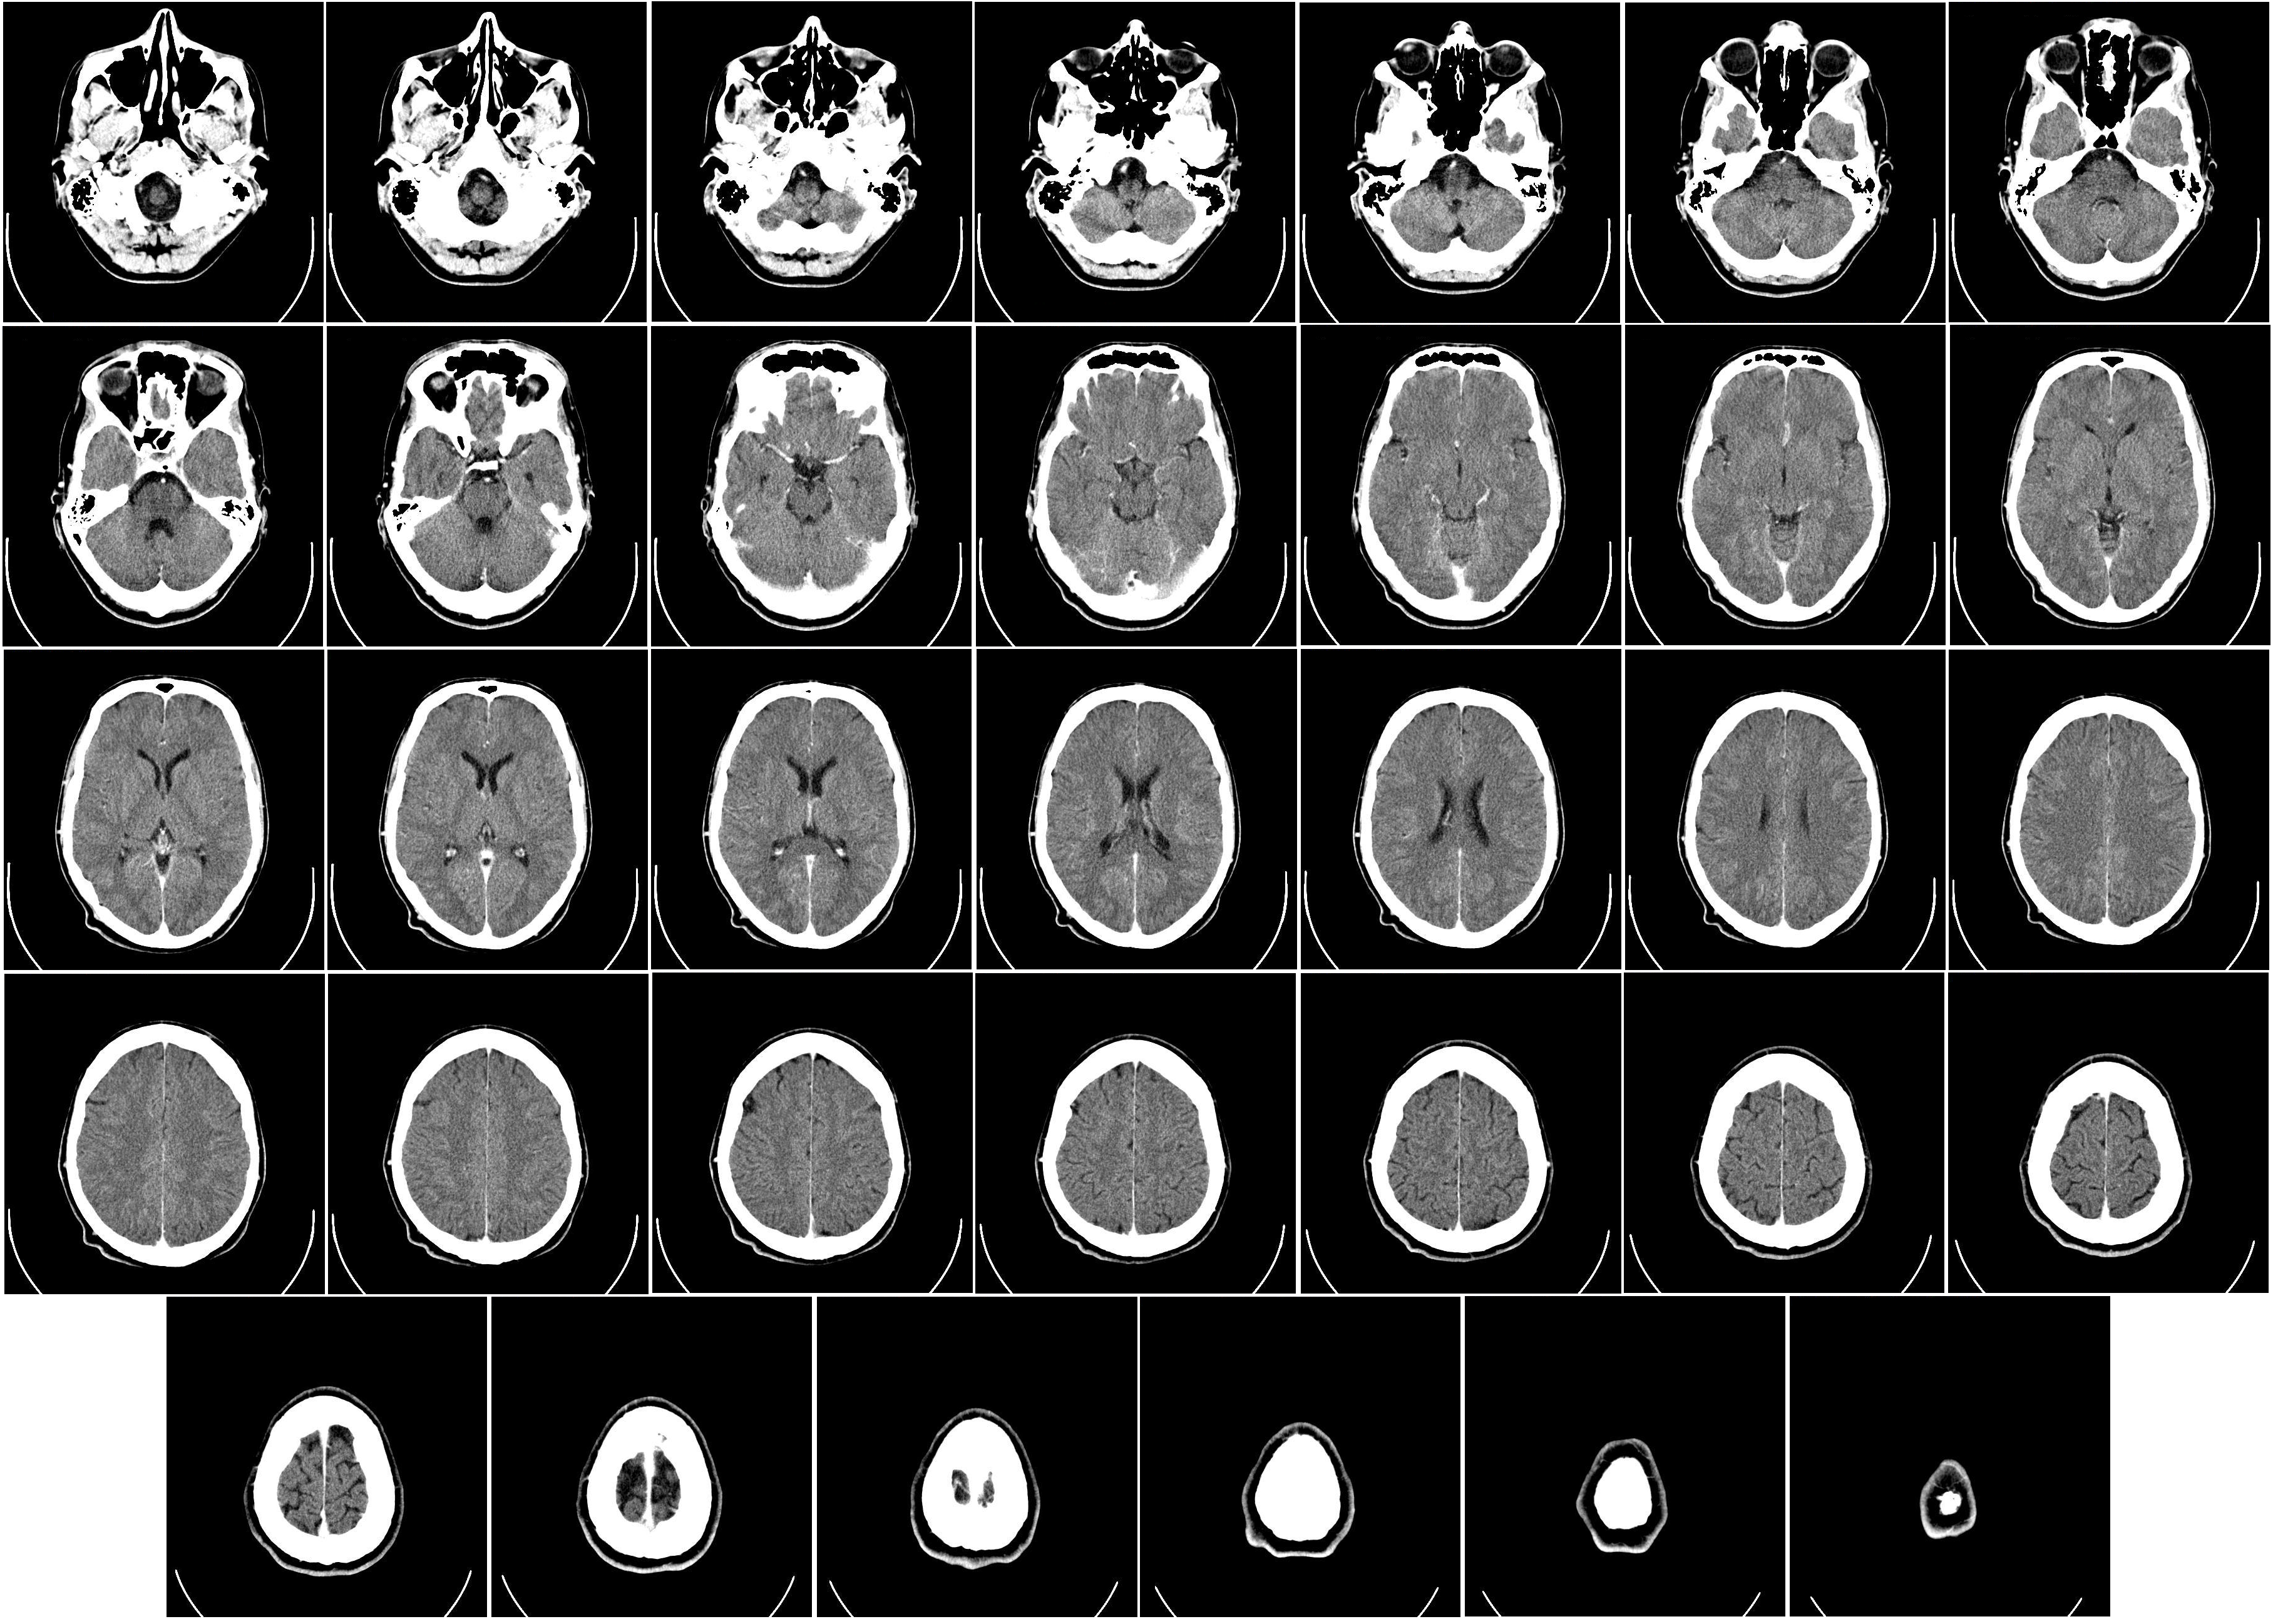
\includegraphics[width=.6\textwidth]{images/ct}
	\end{center}
\end{frame}

\begin{frame}
	\frametitle{1987: 3D}
	3D rendering for surgery planning
	\begin{itemize}
		\item Marching Cubes/Isosurfaces (CT)
		\item ray casting
	\end{itemize}
	\begin{center}
		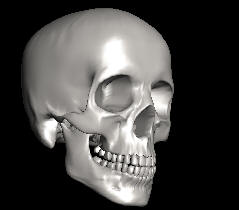
\includegraphics[width=.4\textwidth,height=.4\textheight]{images/marching}
	\end{center}
\end{frame}

\begin{frame}
	\frametitle{Illustrative:} %(Zachow et al. 2009):
	\begin{itemize}
		\item create renditions that consider perceptual abilities of humans
		\item non-photorealistic rendering
		\item for example: boundary enhancement, transfer-functions based on
gradients
	\end{itemize}
	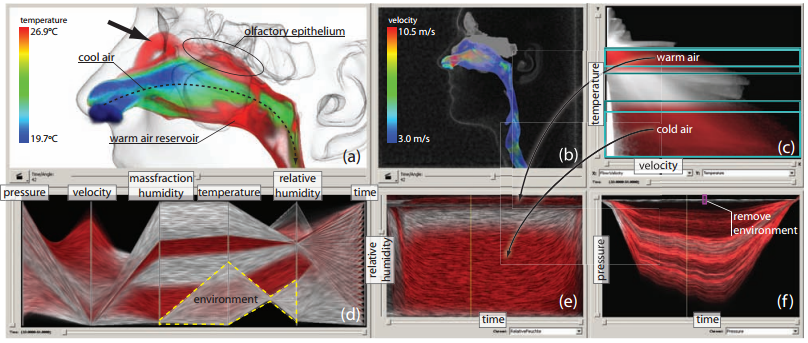
\includegraphics[width=\textwidth]{images/nose}
\end{frame}

\section{Ongoing Challenges}

\begin{frame}
	\frametitle{Ongoing Challenges}
\end{frame}

\begin{frame}
	\frametitle{Mappings and Reformations:}
		This area is still not done;
	\begin{itemize}
		\item standardized mapping of higher dimensions to lower dimension
		\item greatly facilitates interpretation of data
		\item enables study with minimum interaction
	\end{itemize}
	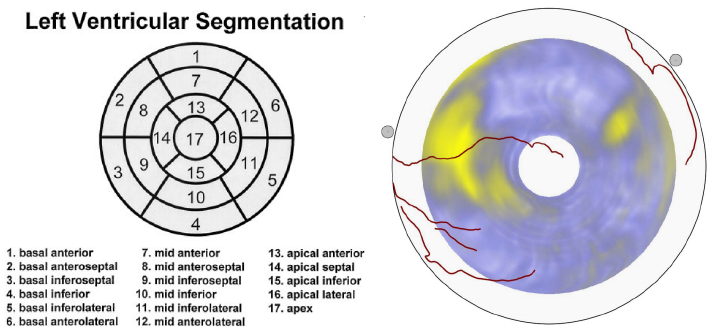
\includegraphics[width=\textwidth]{images/heart}
\end{frame}

\begin{frame}
	\frametitle{Reformative:} % - colon unfolding (Tietjen et al. 2005):
	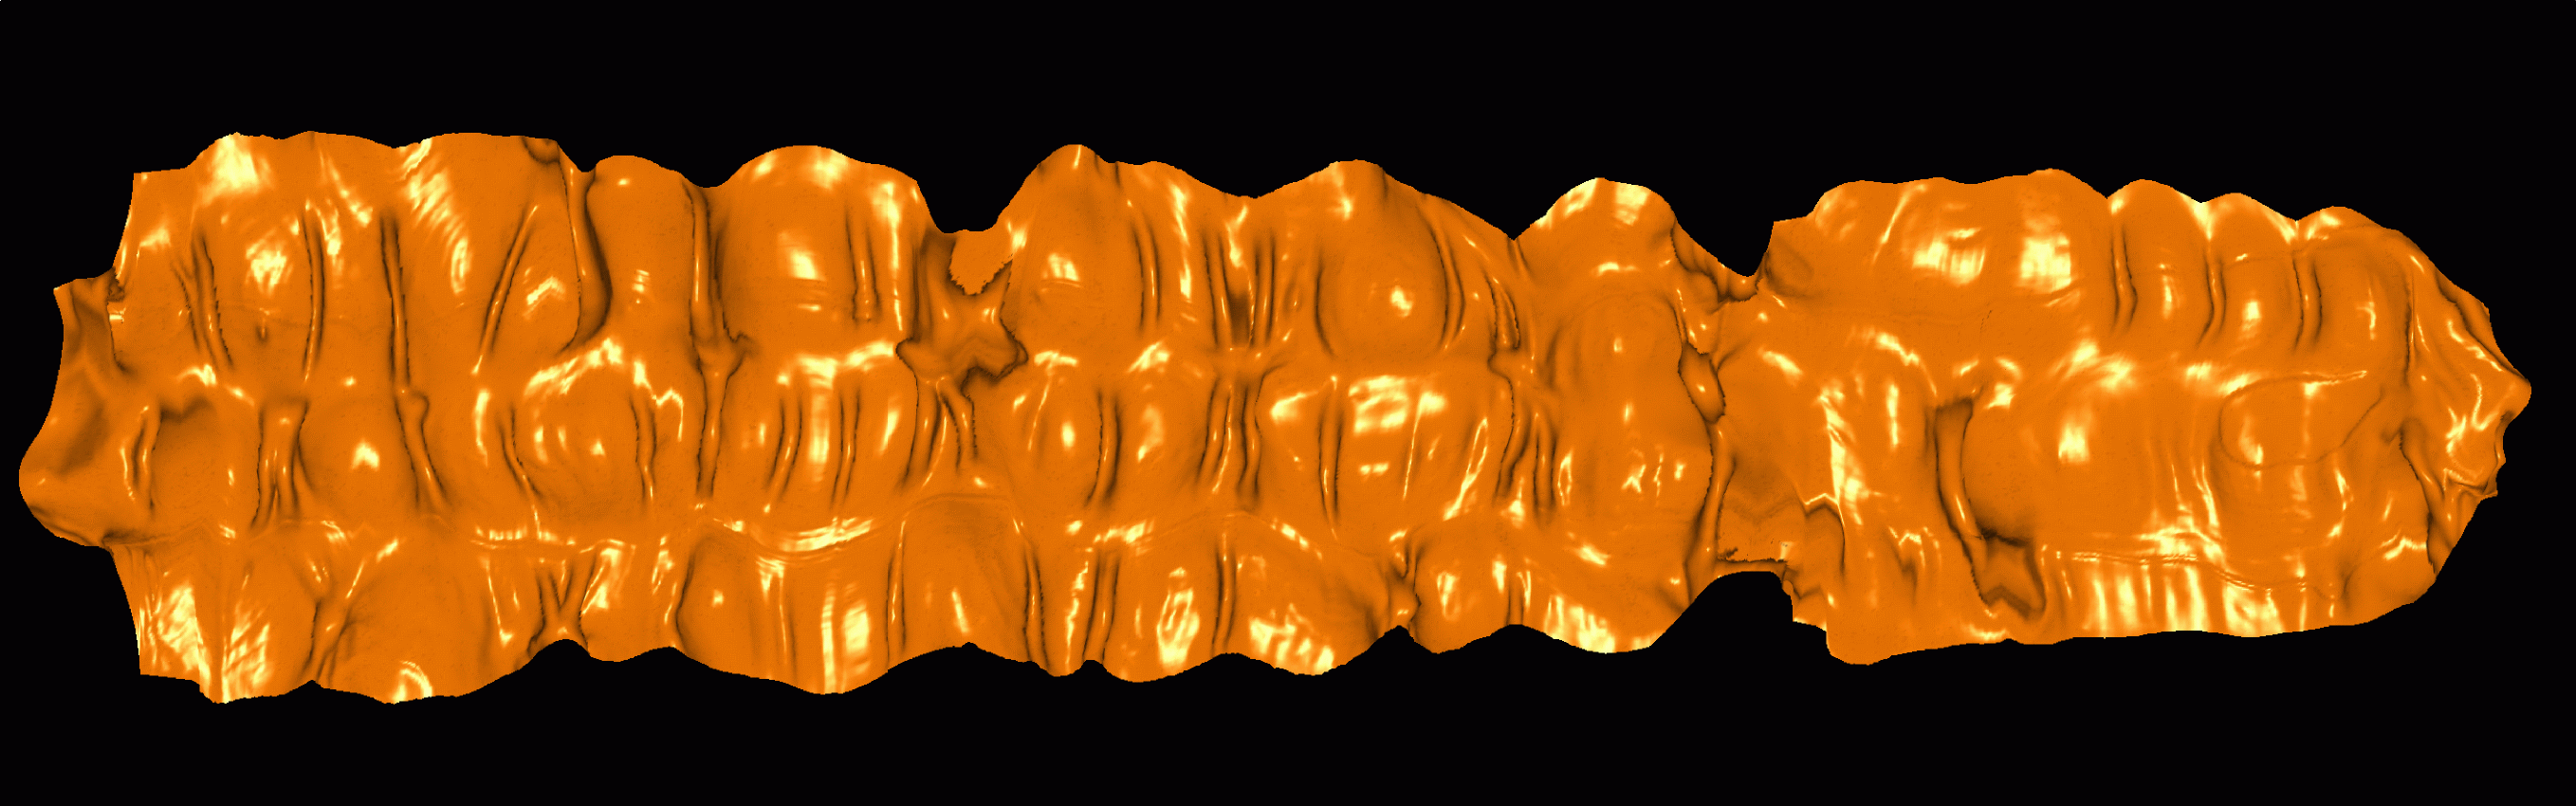
\includegraphics[width=\textwidth]{images/colon}
\end{frame}

\begin{frame}
	\frametitle{Topological methods}
	\begin{itemize}
		\item methods to standardize the data would help
	\end{itemize}
\end{frame}


\section{Advances}

\begin{frame}
	\frametitle{Advances}
\end{frame}

\begin{frame}
	\frametitle{Advances}
		\begin{itemize}
			\item advances in (scanning) equipment and computing power
			\item increase in dimensionality of the data
			\item data is cheaper (so there is more)
			\item new challenges and new opportunities
		\end{itemize}
\end{frame}

%\section{More Complexity}
%\begin{frame}
%	\frametitle{More dimensions}
%	Higher dimensional data due to:
%	\begin{itemize}
%		\item Time-variance
%		\item Multi-field (DTI, tensors)
%		\item Simulation
%		\item Multiple sources
%			\begin{itemize}
%				\item Multi-subject
%				\item Multi-modal
%			\end{itemize}
%	\end{itemize}
%\end{frame}

%\begin{frame}
%	\frametitle{Time-variance}
%	E.g.
%	\begin{itemize}
%		\item fMRI
%		\item Progress of a disease
%		\item Cardiovascular system
%	\end{itemize}
%\end{frame}

%\section{Coping with complexity}
%\begin{frame}
%	\frametitle{More dimensions}
%	\textbf{Solutions:}\\
%	Add interactivity:
%	\begin{itemize}
%		\item Multi-touch devices
%	\end{itemize}
%	Improved visualizations:\\
%	\begin{itemize}
%		\item Illustrative visualizations
%		\item Mappings \& Reformations
%	\end{itemize}
%	versus
%	\begin{itemize}
%		\item Hyper-realism
%	\end{itemize}
%\end{frame}


\subsection{Increase in Dimensionality}
\begin{frame}
	\frametitle{Increase in Dimensionality}
\end{frame}

%\begin{frame}
%	\frametitle{Time-variance}
%	E.g.
%	\begin{itemize}
%		\item fMRI
%		\item Progress of a disease
%		\item Cardiovascular system
%	\end{itemize}
%\end{frame}

\begin{frame}
	\frametitle{2001: 4D}
	Representation of \textbf{time-variance}:
	\begin{itemize}
		\item Tory et al. (2001) use isosurfaces to visualise MS lesions over
			\textbf{time} (MRI)
	\end{itemize}
	\begin{center}
		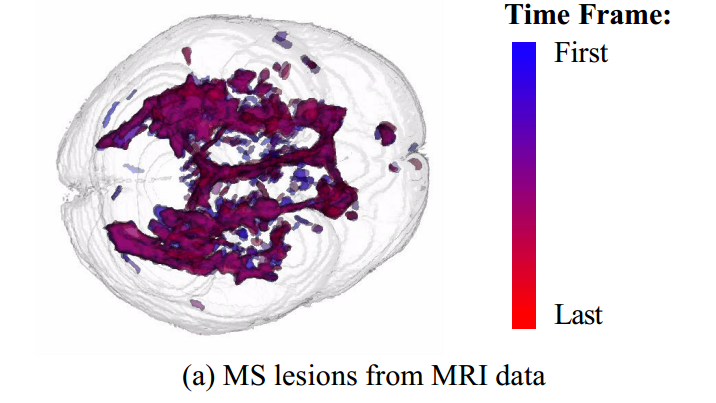
\includegraphics[width=.8\textwidth]{images/ms_time}
	\end{center}
\end{frame}

\begin{frame}
	\frametitle{Advances in data acquisition} % 2.3
	Diffusion Tensor Imaging (DTI), an MRI-based acquisition modality
	\begin{itemize}
		\item able to capture presence and orientation of fibrous structures
(e.g. muscles)
		\item first examples of natively multi-field medical data %(multiple parameters over
the same spatio temporal domain)
	\end{itemize}
	Representing \textbf{multi-modal} DTI data with \textbf{glyphs} was first
	done by Basser et al. in 1994:
	\begin{center}
		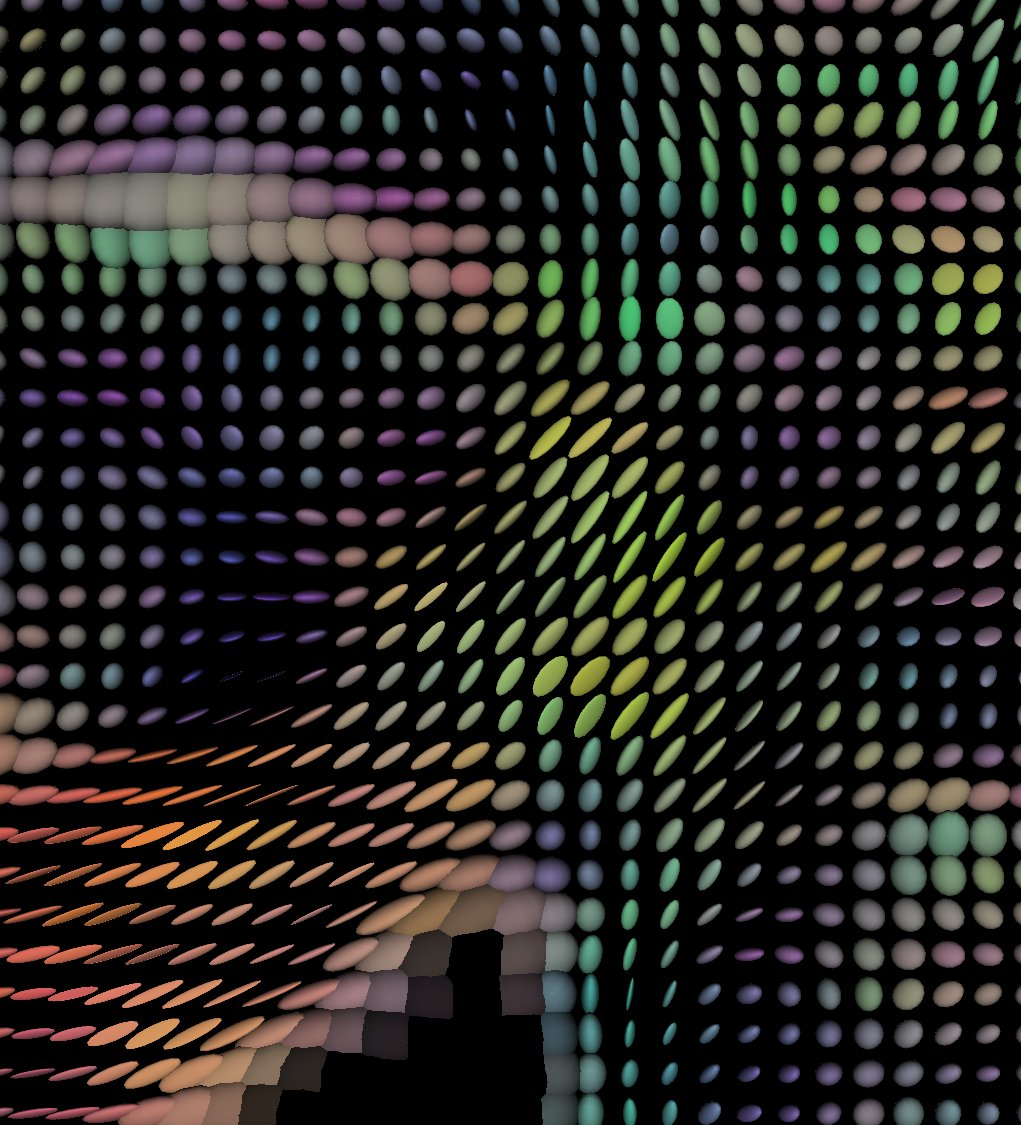
\includegraphics[width=.4\textwidth]{images/dti}
	\end{center}
\end{frame}

\begin{frame}
	\frametitle{DTI:}
	Represented as a spatial colour map:
	\begin{center}
		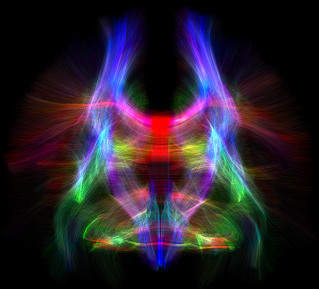
\includegraphics[width=.6\textwidth]{images/tractography}
	\end{center}
\end{frame}

\begin{frame}
	\frametitle{Population Imaging}
	\begin{itemize}
		\item thousands of patients scanned regularly over a period of years
		\item find hypotheses by looking at the data
		\item requires new kind of visualization
	\end{itemize}
\end{frame}

\subsection{With great computing power comes great medical visualization}
\begin{frame}
	\frametitle{With great computing power comes great medical visualization}
\end{frame}

\begin{frame}
	\frametitle{Illustrative Simulations:}
		With more computational power:
		\begin{itemize}
			\item illustrative visualizations can now be simulated
			\item complex simulations can show results of operations
		\end{itemize}
\end{frame}

\begin{frame}
	%\frametitle{With great computing power comes great medical visualization}
	\frametitle{Realism:}
		With more computational power:
	\begin{itemize}
		\item photo-realism
		\item hyper-realism (visual art)
		\item additional realistic details convey info better?
		\item should be explored!
	\end{itemize}
\end{frame}

\begin{frame}
	\frametitle{Realism:}
	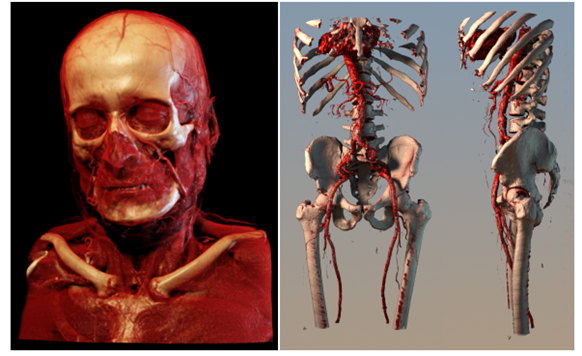
\includegraphics[width=\textwidth]{images/medical_visualisation}
\end{frame}

\begin{frame}
	\frametitle{Realism:}
	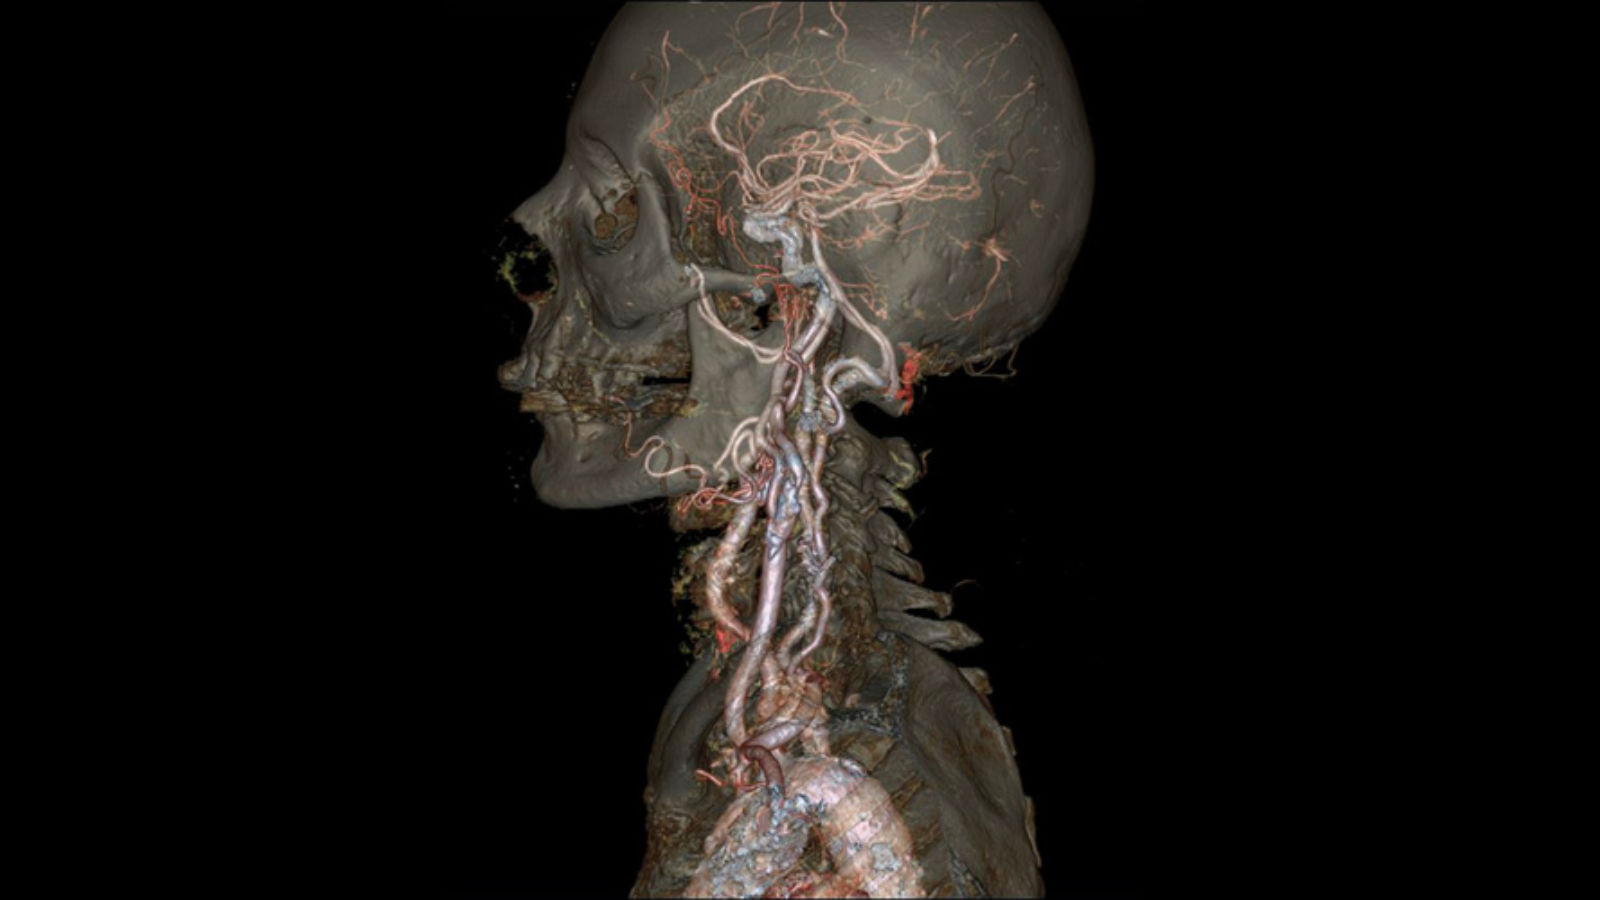
\includegraphics[width=\textwidth]{images/realistic_transparent}
\end{frame}


\subsection{Now Also Possible}
\begin{frame}
	\frametitle{Now Also Possible}
\end{frame}

\begin{frame}
	\frametitle{Heterogeneous display and computing devices:}
	\begin{itemize}
		\item mobile phones have more memory and CPU
		\item doctors already can operate mobile phones
		\item accessible everywhere
	\end{itemize}
\end{frame}

\begin{frame}
	\frametitle{Interactive image segmentation:}
	\begin{itemize}
		\item automatic segmentation is difficult, differences in:
			\begin{itemize}
				\item autonomy
				\item pathology
				\item data acquiring method
			\end{itemize}
		\item combine image analysis, graphics and interaction
	\end{itemize}
\end{frame}

\section{Conclusion}
\begin{frame}
	\frametitle{Conclusion}
\end{frame}

\begin{frame}
	\frametitle{Conclusion}
	\begin{itemize}
		\item Medical visualization has been around for quite some time
		\item New equipment offer new challenges
		\item Lots of possibilities
	\end{itemize}
\end{frame}


%\section{Future Complexity}
%\begin{frame}
%	\frametitle{More dimensions}
%	Higher dimensional data due to:
%	\begin{itemize}
%		\item Time-variance
%		\item Multi-field (DTI, tensors)
%		\item \textbf{Simulation}
%		\item Multiple sources
%			\begin{itemize}
%				\item \textbf{Multi-subject}
%				\item Multi-modal
%			\end{itemize}
%	\end{itemize}
%\end{frame}
%
%\section{Future Solutions}
%\begin{frame}
%	\frametitle{More dimensions}
%	\textbf{Solutions:}\\
%	Add interactivity:
%	\begin{itemize}
%		\item \textbf{Multi-touch devices}
%	\end{itemize}
%	Improved visualizations:\\
%	\begin{itemize}
%		\item \textbf{Illustrative visualizations}
%		\item Mappings \& Reformations
%	\end{itemize}
%	versus
%	\begin{itemize}
%		\item \textbf{Hyper-realism}
%	\end{itemize}
%\end{frame}


\end{document}
% vim: spell
